\documentclass[a4paper,10pt]{article}
\usepackage[utf8]{inputenc}
\usepackage[frenchb]{babel}
\usepackage{graphicx}
\renewcommand*\thesection{\arabic{section}}

%opening
\title{Resolution de problème - Problème des N-Reines}
\author{Jean-Baptiste Dalle}
\date{\today}

\begin{document}

\maketitle

\newpage

\tableofcontents

\newpage

\section{Introduction}

Dans le cadre de l'option résolution de problème du Master 1 Informatique, j'ai eu à développer différents algorithme de résolution permettant de trouver une solution au problème des N-Reines.

Les algorithmes implémentés sont regroupé en regroupés en deux catégories : d'une part, la recherche locale, visant à construire un plateau et à en corriger les conflits au fur et à mesure, et d'une autre part, les algorithmes de programmation par contraintes, visant à placer au fur et à mesure les reines pour atteindre la meilleure solution.

Après avoir développé les différents algorithmes, je me suis attelé à leur optimisation afin d'obtenir de meilleurs temps. Les performances de chaque algorithme sont résumées dans les annexes.

\section{Structure de données}

Avant de m'atteler à la résolution de ce problème, j'ai du mettre en forme le problème des N-Reines de manière à le mettre sous forme d'un CSP.

Une instance du problème des N-Reines se caractérise par le choix de n qui correspond au nombre de reines, de ligne et de colonne. Ainsi, le problème initial nommé problème des 8-Reines est une instance du problème des N-Reines où n vaux 8.

On doit donc poser sur un plateau de taille n*n, n reines représentées par des variable xi avec $i \in {1,..,n}$. Une reine xi se trouve donc sur la ligne i et sa valeur correspond à la colonne où elle est placée. De plus, le placement des reines est régi par certaines contraintes : 

\begin{itemize}
 \item $xi \neq xj$ : Cette contrainte permet d'empêcher deux reines de se trouver sur la même colonne.
 \item $\mid xi - i\mid  \neq  \mid xj - j\mid$ : Cette contrainte permet d'empêcher deux reines de se trouver dans une même diagonale.
\end{itemize}

De manière implicite, chaque reine étant définie par son numéro de ligne, on sait que deux reines ne peuvent se trouver sur la même ligne. Cela correspond donc à une troisième contrainte, mais qui n'est pas utile dans ma représentation.

J'ai décidé d'implémenter ce problème en utilisant le langage Java et ait donc représenté ce problème sous forme d'objet (cf : NReine.java). Une instanciation du problème des N-Reines contient donc un tableau de n cases, chaque case représentant une reine. Une case contenant la valeur null correspond à une reine non encore placée. Une case contenant une valeur quelconque correspond à une reine placée dans cette colonne.

Initialement, j'avais décidé d'implémenter une méthode effectuant la vérification des contraintes entre toutes les reines posées mais cette façon de faire a été modifiée de manière à améliorer les performances de mes algorithmes (cf : 3.2. Optimisation)

\section{Recherche locale}

Comme expliqué précédemment, cette option fut divisée en deux. La première partie concerne donc la résolution par recherche locale. J'ai donc implémenté un algorithme de recherche locale utilisant la méthode du recuit simulé.

\subsection{Implementation}

La recherche consiste à tenter d'améliorer une solution en gardant en mémoire la meilleure solution actuelle. Cependant, arrivé à un certain point, il n'existe plus de solution améliorante. Dans ce but, le recuit simulé permet, suivant une probabilité décroissant au fur et à mesure de l'algorithme, de choisir une solution non améliorante.

Ainsi, lorsqu'une solution est envisagée, si elle n'améliore pas la solution, on la choisit si un nombre tiré aléatoirement est inférieur à l'exponentielle de la différence en nombre de conflit divisé par la température actuelle. La température décroissant à chaque tour de boucle, on a donc de moins en moins de chance de choisir une solution non-améliorante.

Mon implémentation cependant ne s'arrête que lorsqu'une solution a été trouvée. En effet, l'algorithme général s'arrête soit quand la solution a été trouvée, soit quand la température atteint une certaine valeur. Or, le problème des N-Reines comporte toujours une solution lorsque n est supérieur à 4. Mon modèle n'autorisant pas les instances pour lesquelles n est inférieur à 4, il existe donc toujours une solution.

\subsection{Optimisation}

Initialement, mon implémentation permettait de trouver une solution pour l'instance 500-Reine en environ 50s. N'étant pas satisfait de ces performances, je me suis attelé à optimiser mon algorithme ainsi que ma structure de données. Une des premières améliorations apportées fut la mise à jour des contraintes. En effet, ma première formulation du csp était composé de deux contraintes pour les diagonales : $xi - xj  \neq  i - j$ et $xj - xi  \neq  i - j$. Par simplification de celles-ci, je suis arrivé sur la contrainte $\mid xi - xj\mid \neq \mid i - j\mid $.

Une fois cette optimisation faite, je me suis attelé à l'amélioration du calcul des conflits. Initialement, le calcul concernait tout le plateau. A chaque itération, je vérifiais les conflits entre toutes les reines. Evidemment, cette manière de faire était contre-productive et exponentielle. Plutôt que de recalculer les conflits à chaque fois, j'ai mémorisé la liste de ceux-ci. Puis, a chaque déplacement de reine, j'ai mis à jours la liste de conflit suivant la nouvelle position.

Cependant, cette solution restait peu performante. Finalement, je me suis rendu compte que la représentation sous forme d'objet des erreurs était le problème. J'ai amélioré ce mécanisme en ne conservant que le nombre de conflit. Ainsi, lorsqu'un mouvement est effectué, on peut facilement savoir le nombre de conflit entre la reine qui va être déplacée et les autre, réduire le nombre de conflit de ce chiffre, déplacer la reine puis incrémenter le nombre de conflit avec le nouveau chiffre.

N'ayant ainsi plus qu'un entier à la place d'une liste d'objet erreur, les performances de mon algorithme s'en sont retrouvé grandement améliorées, pouvant désormais placer résoudre le problème 2000-Reines en 6 secondes et ayant poussé jusqu'au problème 7000-Reines en moins de 40 secondes.

\section{Programmation par contrainte}

La seconde partie du cours concerne la programmation par contrainte. Durant cette partie, le but a été d'implémenter différents algorithmes visant à construire peu à peu une solution répondant au problème (ici des N-Reines).

\subsection{Back Tracking}

Le premier algorithme implémenté dans le cadre de la programmation par contrainte est celui du Back Tracking. A chaque étape, on choisit une des reines, que l'on place dans chaque emplacement possible. Si l'emplacement est sûr, on continue de dérouler l'algorithme avec la reine suivante. Lorsque toutes les positions ont été testées, si la solution n'a pas été trouvée, on revient à la reine précédente pour tester l'emplacement suivant.

Comme évoqué pour la recherche locale, pour tout problème avec n supérieur ou égale à 4, il existe une solution, l'algorithme renvoi donc toujours une solution. Dans le cas général, une fois toutes les branches testées, il est possible qu'il n'y ait pas de solution.

Néanmoins, cet algorithme n'est pas le plus efficace qui soit. En effet, à chaque itération, chaque reine est testée sur chacune des positions. Dans l'algorithme suivant, nous verrons comment améliorer cet aspect.

\subsection{Forward Checking}

Ce second algorithme est assez ressemblant au Back Tracking mais diffère en un point majeur : plutôt que, pour chaque reine, essayer chaque colonne, on ne testera que les positions étant toujours valides par rapport aux dames déjà placées. Cela signifie entre autre que chaque position testée est toujours supposée valide étant donné que les positions invalides ont déjà été supprimées.

Dans le cas du problème des N-Reines, cet algorithme est assez peu efficace. En effet, les contraintes sont toutes des contraintes de différences, le domaine de chaque reine est donc peu réduit. En effet, lorsqu'une reine est posée, on va réduire le domaine d'une autre reine d'une, deux ou trois positions (horizontale et éventuellement deux diagonales). Le domaine s'en retrouve donc assez peu affecté par rapport à des contraintes d'égalité par exemple qui auraient supprimées toutes les valeurs exemptées une.

\subsection{Arc Consistancy 3}

L'Arc Consistancy est un algorithme permettant de vérifier l'arc consistance de plusieurs variables (ici de plusieurs reines) et ainsi de supprimer du domaine de chaque reine les positions ne respectant pas l'arc consistance.

Cependant, pour les raisons évoquées plus tôt, l'Arc Consistance n'est pas performante pour le problème des N-Reines. En effet, il ne réduit le domaine que des instances 2-Reines et 3-Reines, qui n'ont alors plus de solution.

On comprend donc assez vite qu'AC, bien que peu couteux n'a aucun apport pour ce problème.

\subsection{Heuristique}

Une fois les différents algorithmes implémentés, je me suis attelé à l'implémentation des heuristiques. Ceux-ci permettront de trier les données de différentes manière afin d'obtenir les meilleures performances possibles.

\subsubsection{First find}

Jusqu'à maintenant, j'utilisais l'heuristique First Find : on utilise toujours les valeurs dans l'ordre retourné par l'itérateur. La plupart du temps, cela correspondra à une heuristique minimale (car les liste ont étés peuplées de manière croissante) mais dans le cas du forward checking, l'ordre peut être altéré car, après que le domaine ait été réduit et qu'on doit le restaurer, les variables retirées sont remises en fin de liste.

\subsubsection{Minimimum first}

L'heuristique First find étant implémentée par défaut, je me suis attelée trier de manière à ce que les valeurs soient retourné par ordre croissant. Cette heuristique n'a cependant pas beaucoup amélioré les performances de mes algorithmes, restant sur les même temps d'exécution. 

\subsubsection{Maximum first}

L'heuristique Maximum first consiste à trier dans l'ordre décroissant les valeurs. Cependant, cette nouvelle heuristique n'a toujours pas modifié les performances des algorithmes.

\subsubsection{Random}

Que ce soit pour minimum first ou maximum first, comme les reines seront placées sur les dernières colonnes en premier (ou les premières dans le cas de min first), plus on avance dans l'algorithme, plus on doit parcourir de colonne déjà occupée par une précédente reine.

De manière à briser ce comportement, j'ai développé une heuristique random qui renvoi dans un ordre aléatoire les valeurs. Cette heuristique s'est révélée dans la plupart des cas extrêmement performante car il arrivera souvent que les reines soient placées dans des colonnes non encore occupées par d'autres reines.

Cependant, plus l'instance du problème est grande, plus on risque de tomber sur des cas où le placement posera le même problème que pour l'heuristique min et max first. Ainsi, grâce à cette heuristique, il m'a été possible de résoudre des instances 90-Reines de manière instantanées ou au contraire que le traitement soit trop long pour être terminé.

\subsubsection{Minimum domain size first}

Je me suis finalement attelé à une dernière heuristique, visant à placer en premier les reines disposant du plus petit domaine. Comme le domaine n'est pas réduit par l'algorithme AC3, cette heuristique n'est pas efficace pour l'algorithme du back tracking car le domaine reste intact au fil de l'exécution et les reines sont donc retournées dans l'ordre normal.

Toutefois, dans le cas du forward checking, cette heuristique s'est révélée extrêmement performante. En effet, lorsqu'une reine n'aura plus que quelques emplacements possibles, on la posera en priorité, évitant ainsi de placer une reine avec beaucoup de possibilités qui invalidera les reines avec peu de possibilités.

Contrairement à l'heuristique Random cependant, celle-ci fournit de bonne performances jusqu'à un certain point (ici 90-Reines) mais tous les précédentes instances du problème seront résolus presque instantanément.

\subsection{Performance}

En terme de performance, les différents algorithmes implémentés arrivent à résoudre en un temps raisonnable le problème des N-Reines jusqu'à l'instance 31-Reines (l'instance 30-Reines est cependant plus lente à résoudre que l'instance 31-Reines).

Cependant, deux configurations ressortent du lot : L'algorithme Forward Checking couplé aux heuristiques Random ou Min Domain Size (et éventuellement l'algorithme Forward Checking + AC3 qui a les même performances que le Forward Checking simple). Sur ces configurations, il est possible de résoudre le problème des N-Reines jusqu'à l'instance 90-Reines en un temps raisonnable. Au-delà des 90-Reines, l'heuristique Min Domain Size devient trop lente alors que l'heuristique random a de plus en plus de chance d'être très lente.

Une manière d'obtenir des résultats pour des instances un plus grandes pourrait être de tenter de lancer de nombreuse fois le Forward Checking + Random jusqu'à arriver à une solution presque instantanée.

\section{Conclusion}

Au fil de ce projet, j'ai pu développer différents algorithmes permettant de résoudre le problème des N-Reines. La plupart des algorithmes étaient relativement efficaces, mais pour gagner en performance, j'ai eu à optimiser plusieurs parties de mon code. 


Arrivé au terme de ce projet, je me rends cependant compte que les optimisations possibles deviennent limitées et de plus en plus complexes. En conclusion, je pense que, de manière à augmenter davantage les performances, il faudrait modifier la structure même des algorithmes ou en utiliser d'autres. Une autre solution pourrait être de changer de structure de données voire d'abandonner le modèle objet de manière à gagner en performance avec des structures plus efficaces.

\section{Annexe}

\subsection{Annexe 1 - Performance : Recherche locale}
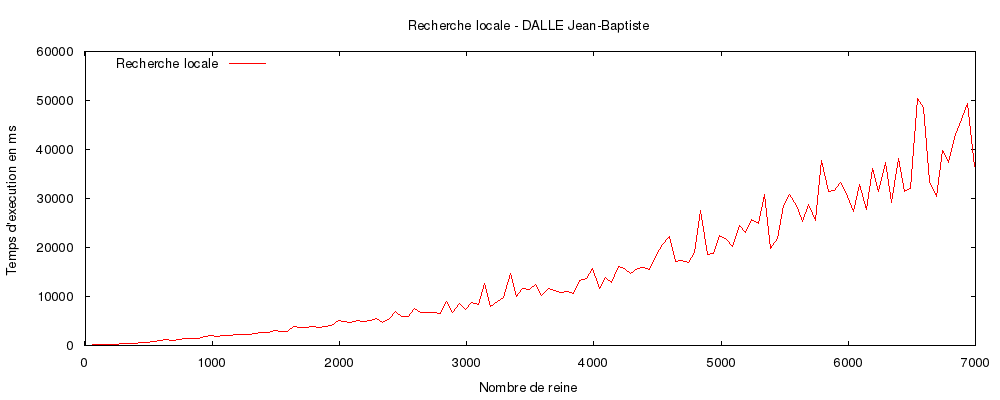
\includegraphics[width=1\textwidth]{Recherche_Locale.png}

\subsection{Annexe 2 - Performance : Programmation par contraintes}
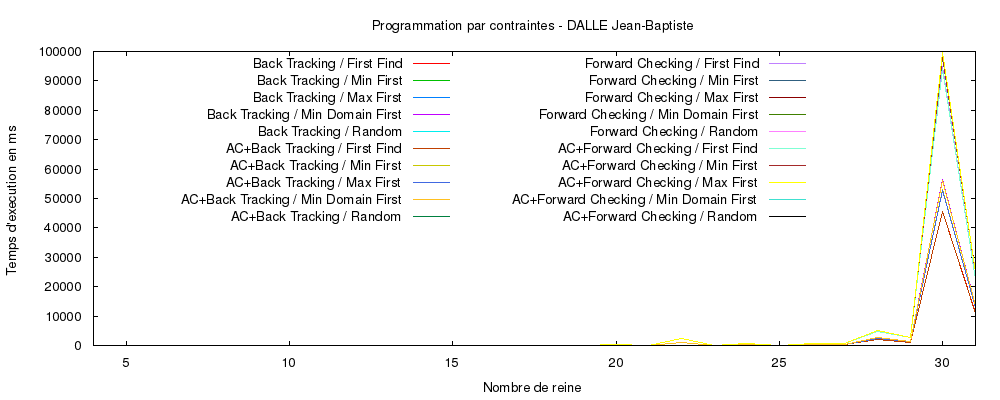
\includegraphics[width=1\textwidth]{Programmation_par_contraintes.png}

\subsection{Annexe 3 - Performance : Programmation par contraintes - Back Tracking}
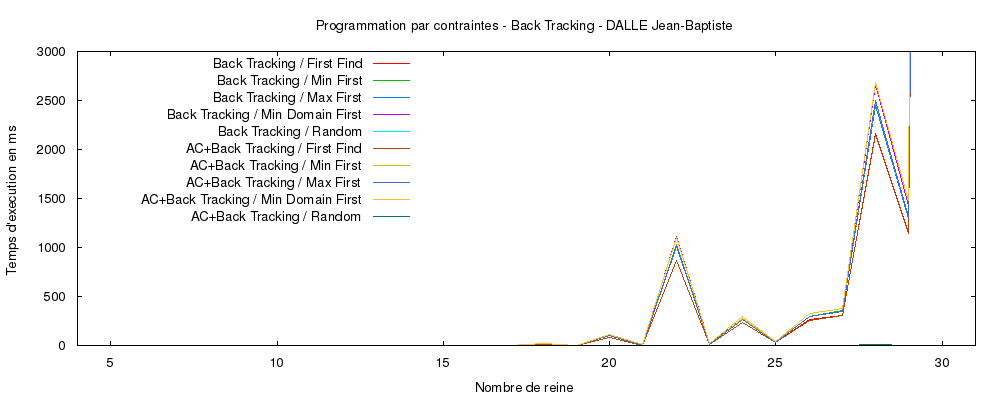
\includegraphics[width=1\textwidth]{Programmation_par_contraintes_-_Back_Tracking.png}

\subsection{Annexe 4 - Performance : Programmation par contraintes - Forward Checking}
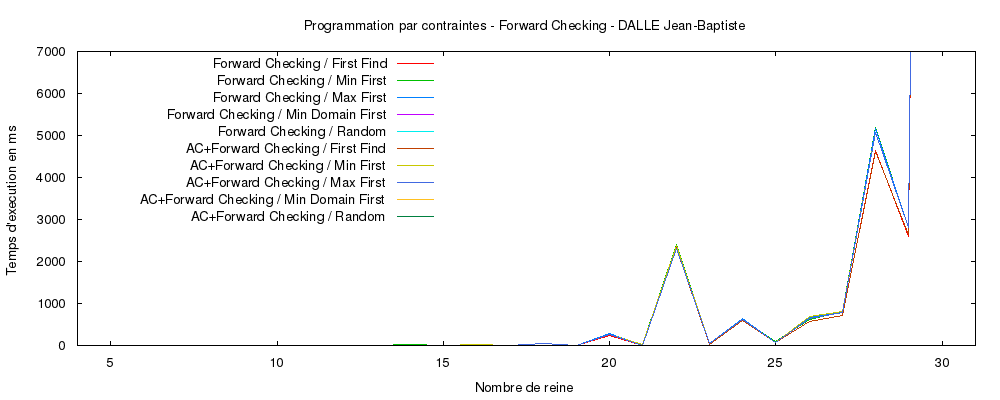
\includegraphics[width=1\textwidth]{Programmation_par_contraintes_-_Forward_Checking.png}

\subsection{Annexe 5 - Performance : Programmation par contraintes - Random et Minimum domaine size}
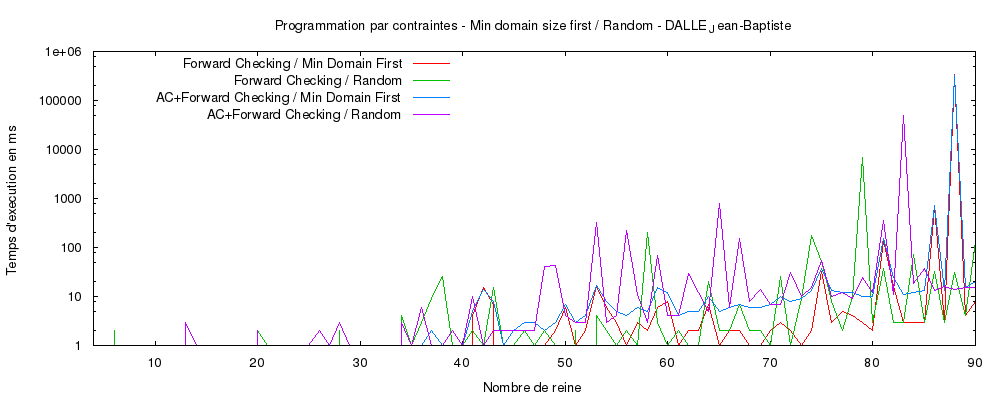
\includegraphics[width=1\textwidth]{Programmation_par_contraintes_-_Random_Min_Domain_Size.png}

\end{document}